\documentclass[letterpaper]{article}
\usepackage{csc-poster}
\usepackage{hyperref}

\begin{document}

\cschead{\emph{To Mock a Mockingbird} Club de Lecture}{}

\cscsubtitle{Partons à l'aventure en logique combinatoire!}
%\cscsubtitle{Ces oiseaux doivent payer pour leur orgueil!}

\emph{To Mock a Mockingbird and Other Logic Puzzles: Including an Amazing Adventure in Combinatory Logic} est un livre par le math\'ematicien et logicien Raymond Smullyan qui contient de nombreuses \'enigmes pour lequel l'auteur est connu. C'est aussi une douce et dr\^ole introduction \`a la logique combinatoire et les m\'etamath\'ematiques li\'ees, fond\'ee sur une m\'etaphore ornithologique \'elabor\'ee.

\vspace{0.75in}
\begin{tabular}{rl}
    \csctimefont Livre: &  \\
    & \\
    \csctimefont Serveur Discord: &
\end{tabular}

\vspace{0.5in}
\begin{center}
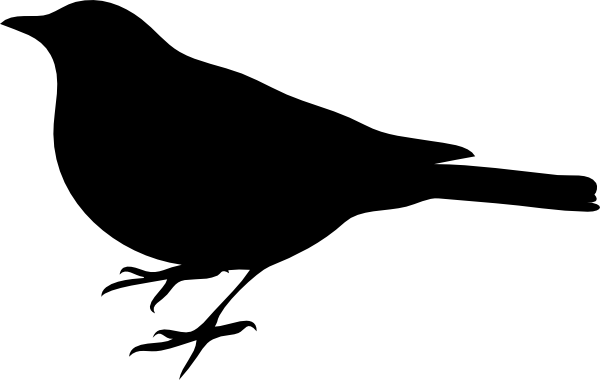
\includegraphics[scale = 0.75]{mockingbird_logo.png}
\end{center}

\cscsubtitle{La prochaine s\'eance commencera en janvier}
\vspace{-15pt}
\cscsubtitle{Ponctualit\'e non n\'ecessaire}
\vspace{-15pt}
\centering \cscsubtitle{\small Tous les jeunes cool le font; ne veux-tu pas \^etre dans le coup}

\raggedleft

\includegraphics[scale = 0.5]{mef_logo.png}
\end{document}
% Thanks to Rebecca Wilson for this translation
